% \chapter{Client-server view (UML Component diagram)}\label{ch:client-server}

% Delete the command below to remove the hints and instructions
\showcsnotes{}

\section{Context diagram}
    TODO: find a way to display the page horizontally with the image covering the whole page. \\

    The context diagram of the client-server view is displayed in figure \ref{fig:cc-context}. \\

    The external components are as follows.
    \begin{itemize}
        \item NotificationDeliveryService: blabla
        \item InfrastructureOwnerClient: blabla
        \item CustomerOrganisationClient: blabla
    \end{itemize}

    \todoinline{
    The context diagram of the client-server view:
    Discuss which components communicate with external components and what these external components represent.
    }

    \begin{figure}[!htp]
    	\centering
    	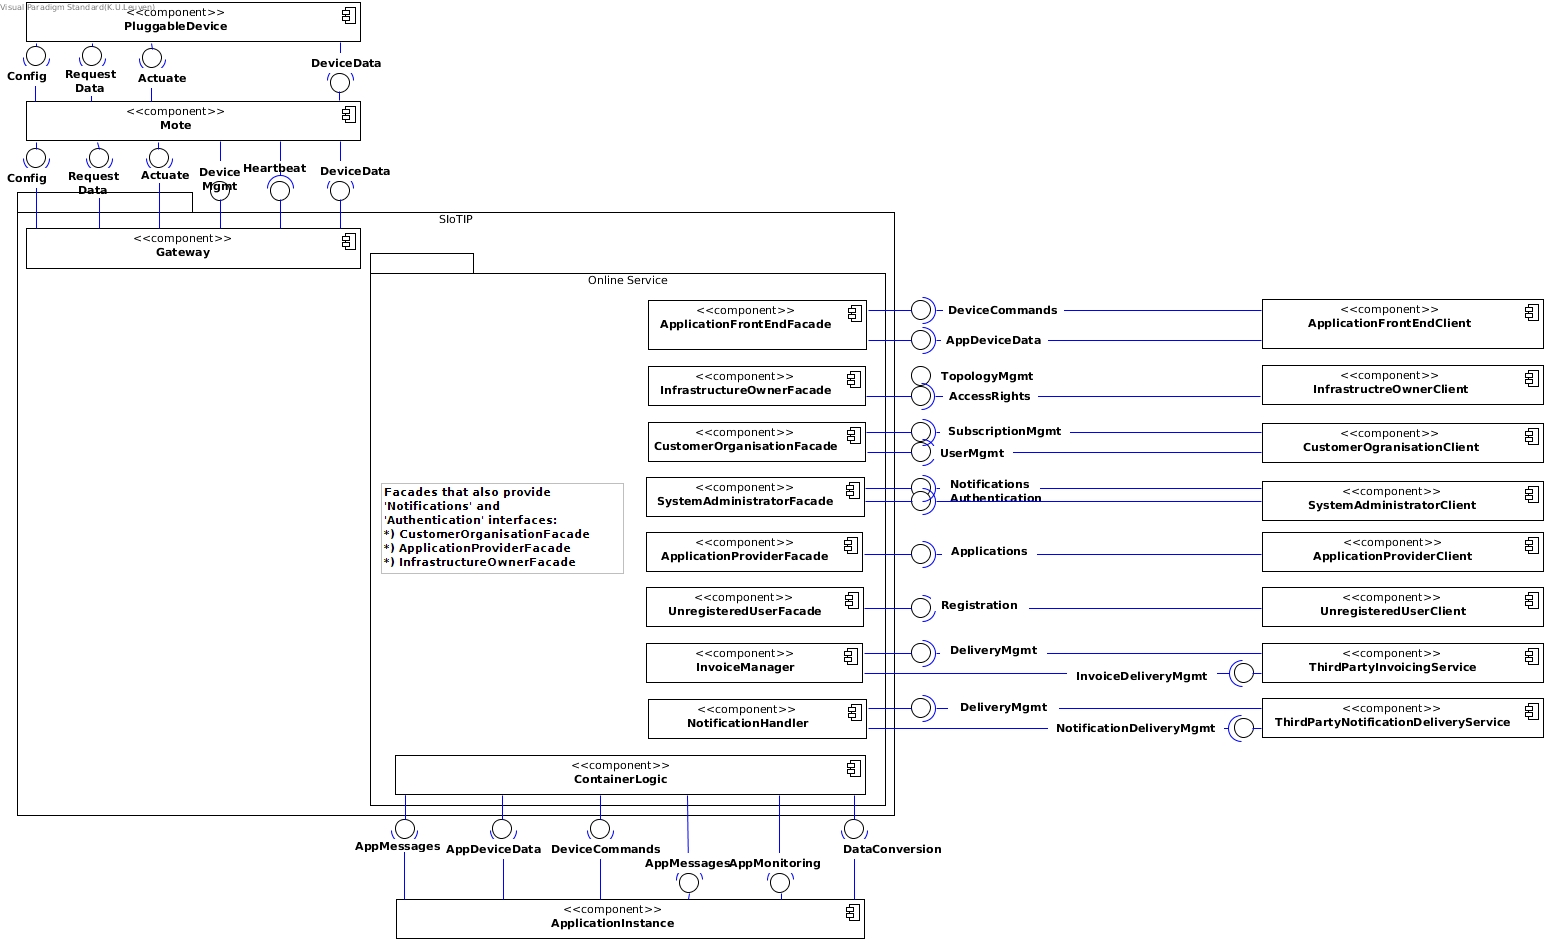
\includegraphics[width=\textwidth]{images/component-CONTEXT}
    	\caption{Context diagram for the client-server view.}\label{fig:cc-context}
    \end{figure}

\section{Primary diagram}
    The primary diagram of the client-server view is displayed in figure \ref{fig:cc-primary}. \\

    \todoinline{The primary diagram and accompanying explanation.}

    \begin{figure}[!htp]
    	\centering
    	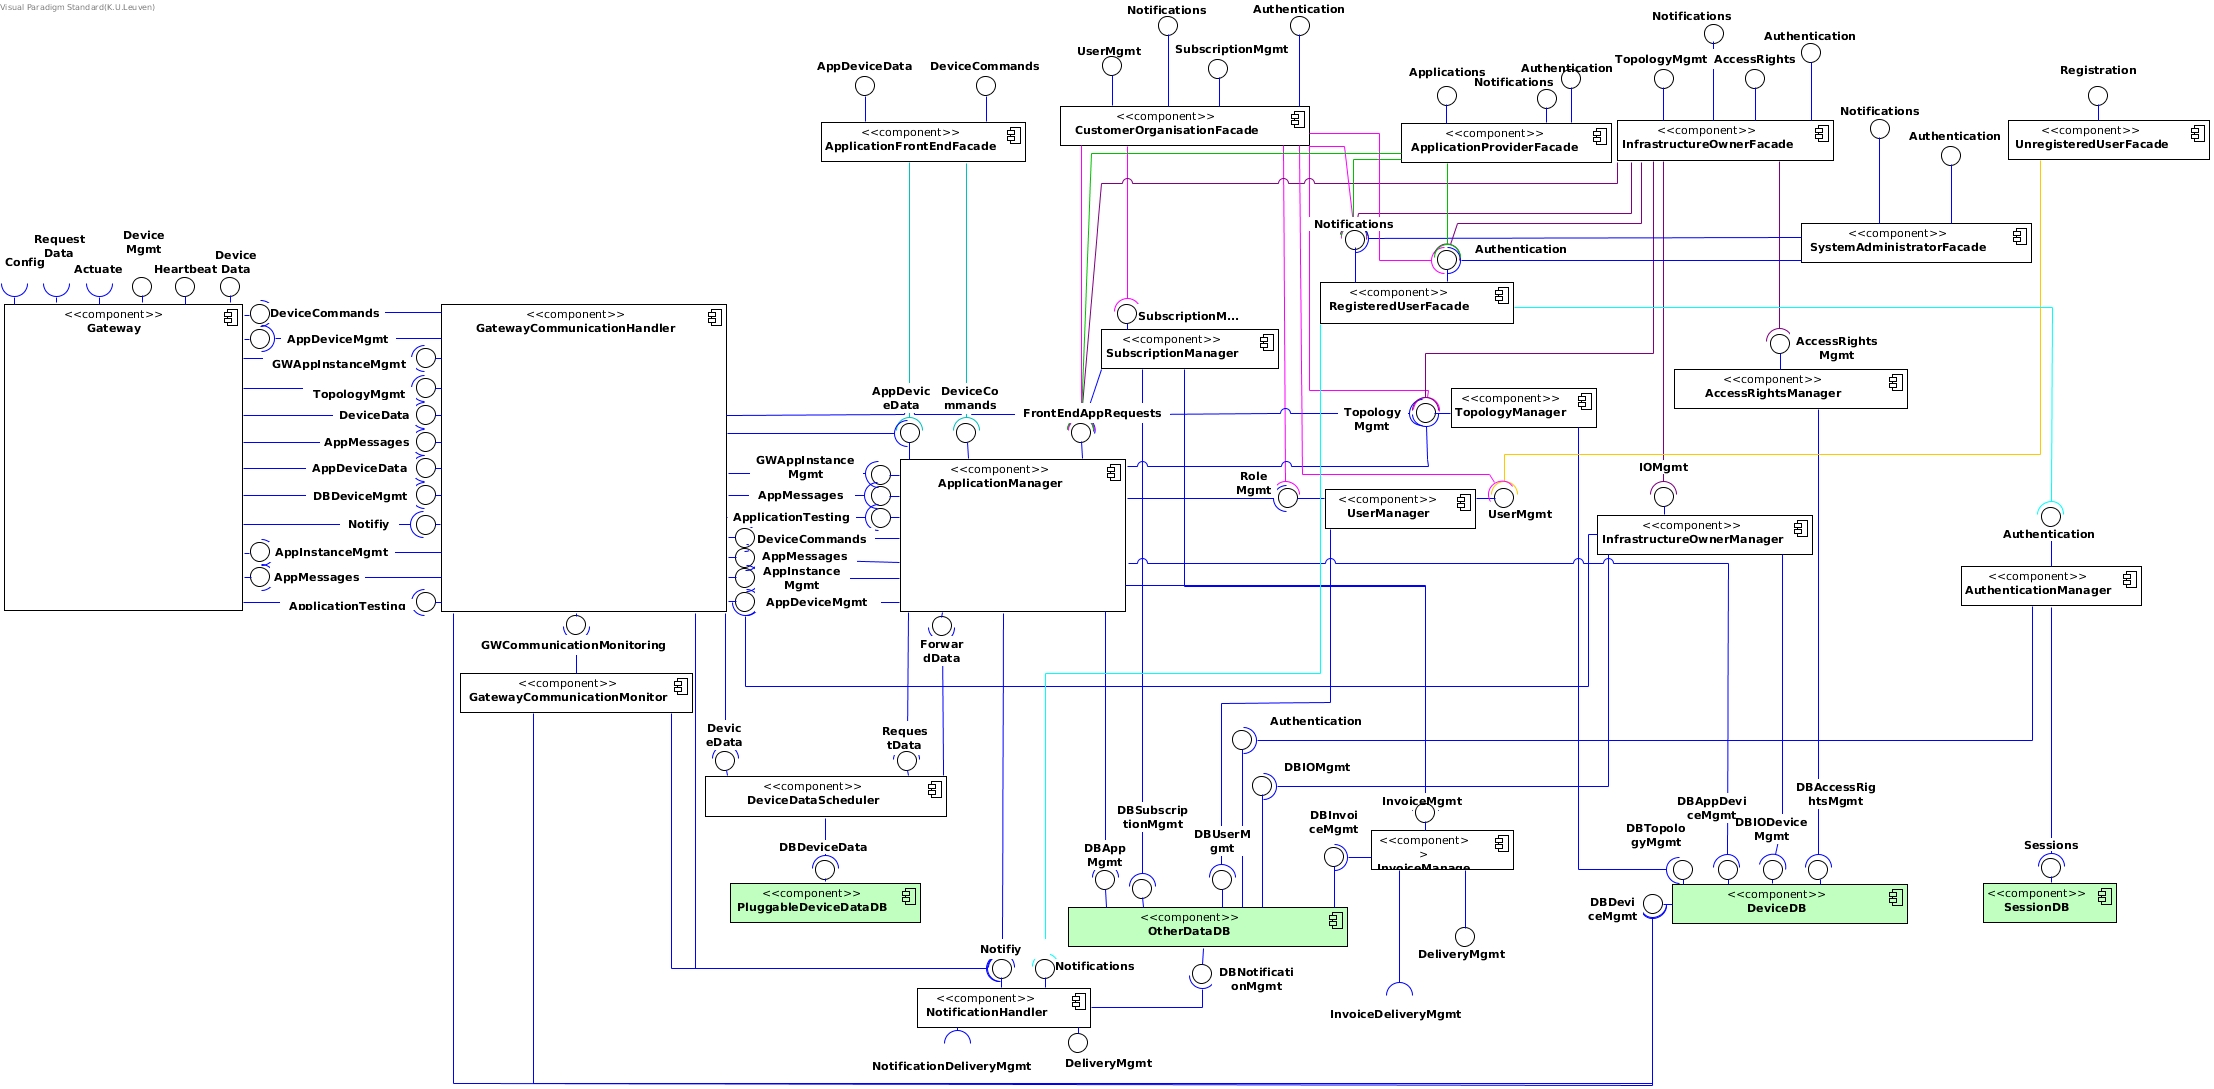
\includegraphics[width=\textwidth]{images/component-PRIMARY}
    	\caption{Primary diagram of the client-server view.}\label{fig:cc-primary}
    \end{figure}
